\section{Capítulo 10 -- Busca e ordenação}

Procurar e ordenar estão entre as tarefas que os computadores mais executam. Toda vez que você procura um contato no celular, filtra produtos pelo menor preço ou vê a classificação de um campeonato, há um algoritmo de busca ou de ordenação trabalhando. Elas também são o lugar ideal para uma pergunta nova: não basta o algoritmo estar certo, ele precisa ser \textbf{rápido o suficiente}. Neste capítulo você vai conhecer as duas buscas fundamentais, a sequencial e a binária, três algoritmos clássicos de ordenação (seleção, bolha e inserção) e uma forma simples de comparar a eficiência de algoritmos contando quantas operações eles fazem.

\subsection{10.1 Busca sequencial}

A forma mais direta de procurar um valor em um vetor é olhar os elementos um por um, do primeiro ao último, até encontrá-lo ou até o vetor acabar. Essa é a \textbf{busca sequencial} (ou linear). A função devolve a \textbf{posição} em que o valor foi encontrado ou, se ele não estiver no vetor, um valor que não pode ser uma posição válida, como $-1$.

\begin{codigo}
\begin{Verbatim}[breaklines=true, breaksymbolleft={}, fontsize=\footnotesize]
#include <iostream>
using namespace std;

int buscaSequencial(const int v[], int n, int x) {
    for (int i = 0; i < n; i++) {
        if (v[i] == x) return i;    // achou: devolve a posição
    }
    return -1;                      // olhou tudo e não achou
}

int main() {
    int v[] = {42, 7, 19, 73, 4, 56, 23};
    int x;
    cout << "Procurar: ";
    cin >> x;
    int pos = buscaSequencial(v, 7, x);
    if (pos >= 0) cout << "Achou na posição " << pos << endl;
    else cout << "Não encontrado" << endl;
    return 0;
}
// 73 -> Achou na posição 3       10 -> Não encontrado
\end{Verbatim}
\end{codigo}

Em Portugol, sem um \texttt{return} no meio do laço, a busca usa uma variável que guarda a posição encontrada e faz parte da condição do \texttt{enquanto}: o laço para quando acha o valor ou quando os elementos acabam.

\begin{codigo}
\begin{Verbatim}[breaklines=true, breaksymbolleft={}, fontsize=\footnotesize]
algoritmo "BuscaSequencial"
var
   v: vetor[1..7] de inteiro
   i, x, pos: inteiro
inicio
   para i de 1 ate 7 faca
      escreva("Elemento ", i, ": ")
      leia(v[i])
   fimpara
   escreva("Procurar: ")
   leia(x)
   pos <- 0                   // 0: ainda não encontrado
   i <- 1
   enquanto (i <= 7) e (pos = 0) faca
      se v[i] = x entao
         pos <- i
      fimse
      i <- i + 1
   fimenquanto
   se pos > 0 entao
      escreval("Achou na posição ", pos)
   senao
      escreval("Não encontrado")
   fimse
fimalgoritmo
\end{Verbatim}
\end{codigo}

A busca sequencial funciona com qualquer vetor, ordenado ou não. O preço é que, no pior caso (o valor está no fim ou não está no vetor), ela olha \textbf{todos} os $n$ elementos. Em um vetor com um milhão de elementos, isso são um milhão de comparações.

\subsection{10.2 Busca binária}

Ninguém procura uma palavra no dicionário lendo da primeira página em diante. Abre-se o dicionário mais ou menos no meio e, conforme a palavra vem antes ou depois da página aberta, descarta-se a metade em que ela não pode estar. A \textbf{busca binária} faz exatamente isso, e por isso só funciona em vetores \textbf{ordenados}.

O algoritmo mantém dois índices, \texttt{ini} e \texttt{fim}, que delimitam a parte do vetor onde o valor ainda pode estar. A cada passo, compara o valor procurado com o elemento do meio dessa parte: se for igual, achou; se o procurado for maior, ele só pode estar à direita do meio; se for menor, só à esquerda. Quando \texttt{ini} passa de \texttt{fim}, a parte ficou vazia, e o valor não está no vetor.

\begin{center}
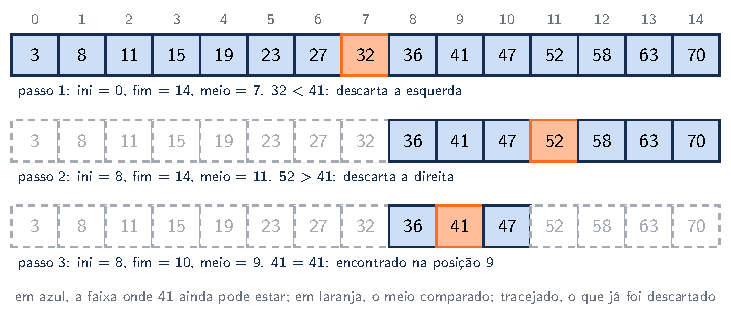
\includegraphics[width=0.9\linewidth,keepaspectratio]{imagens/capitulo-10_binaria.pdf}
\end{center}

\begin{codigo}
\begin{Verbatim}[breaklines=true, breaksymbolleft={}, fontsize=\footnotesize]
#include <iostream>
using namespace std;

int buscaBinaria(const int v[], int n, int x) {
    int ini = 0, fim = n - 1;
    while (ini <= fim) {
        int meio = ini + (fim - ini) / 2;
        if (v[meio] == x) return meio;
        if (v[meio] < x) ini = meio + 1;   // está à direita
        else fim = meio - 1;               // está à esquerda
    }
    return -1;                             // a faixa ficou vazia
}

int main() {
    int v[] = {3, 8, 11, 15, 19, 23, 27, 32, 36, 41, 47, 52, 58,
               63, 70};
    cout << buscaBinaria(v, 15, 41) << endl;   // 9
    cout << buscaBinaria(v, 15, 3) << endl;    // 0
    cout << buscaBinaria(v, 15, 40) << endl;   // -1
    return 0;
}
\end{Verbatim}
\end{codigo}

O meio é calculado como \texttt{ini + (fim - ini) / 2}, e não como \texttt{(ini + fim) / 2}. As duas contas dão o mesmo resultado, mas a segunda pode estourar o limite do \texttt{int} quando os índices são muito grandes, um erro que passou anos despercebido em bibliotecas usadas no mundo inteiro.

A cada passo, a busca binária descarta metade do que resta. Um vetor de 15 elementos precisa de no máximo 4 comparações; um de mil, de 10; um de um milhão, de apenas 20, porque 20 divisões ao meio reduzem um milhão a um único elemento. Em termos matemáticos, o número de passos é cerca de $\log_2 n$.

A busca binária também tem uma versão recursiva natural (Capítulo 9): procurar em uma faixa é olhar o meio e procurar em uma das metades.

\begin{codigo}
\begin{Verbatim}[breaklines=true, breaksymbolleft={}, fontsize=\footnotesize]
int buscaRec(const int v[], int ini, int fim, int x) {
    if (ini > fim) return -1;              // caso base: vazia
    int meio = ini + (fim - ini) / 2;
    if (v[meio] == x) return meio;
    if (v[meio] < x) return buscaRec(v, meio + 1, fim, x);
    return buscaRec(v, ini, meio - 1, x);
}
\end{Verbatim}
\end{codigo}

\subsection{10.3 Quanto custa um algoritmo}

Medir o tempo de um programa com um cronômetro diz pouco, porque o resultado depende do computador, da linguagem e até do que mais estava rodando. Uma medida mais útil é \textbf{contar as operações} básicas que o algoritmo faz, como comparações, em função do tamanho $n$ da entrada, e observar como esse número cresce quando $n$ cresce. Essa é a ideia de \textbf{complexidade} de um algoritmo:

\begin{center}
\begin{tabular}{@{}p{0.13\linewidth}p{0.16\linewidth}p{0.14\linewidth}p{0.2\linewidth}p{0.18\linewidth}@{}}
\toprule
\rowcolor{headergray}
\tblheader{$n$} & \tblheader{sequencial} & \tblheader{binária} & \tblheader{ordenação} & \tblheader{\texttt{sort}} \\
\rowcolor{headergray}
& \tblheader{($n$)} & \tblheader{($\log_2 n$)} & \tblheader{simples ($n^2$)} & \tblheader{($n \log_2 n$)} \\
\midrule
10 & 10 & 4 & 100 & 33 \\
\rowcolor{rowgray} 1.000 & 1.000 & 10 & 1 milhão & 10 mil \\
1 milhão & 1 milhão & 20 & 1 trilhão & 20 milhões \\
\bottomrule
\end{tabular}
\end{center}

A tabela mostra o número aproximado de operações. Os valores exatos importam menos que a forma do crescimento. Quando $n$ fica mil vezes maior, a busca sequencial fica mil vezes mais lenta, enquanto a binária precisa de só 10 passos a mais. Já os algoritmos de ordenação simples deste capítulo, que crescem com $n^2$, ficam um \textbf{milhão} de vezes mais lentos. A um bilhão de operações por segundo, ordenar um milhão de números leva 20 milissegundos com um algoritmo $n \log n$, e mais de 15 minutos com um algoritmo $n^2$. Os cientistas da computação escrevem essas formas de crescimento com a notação $O$ (``ó grande''): $O(n)$, $O(\log n)$, $O(n^2)$, $O(n \log n)$.

\subsection{10.4 Ordenação por seleção}

A \textbf{ordenação por seleção} é a forma como muita gente ordena cartas na mão: encontra a menor e a põe em primeiro lugar; entre as que sobraram, encontra a menor e a põe em segundo; e assim por diante. Cada passada pelo vetor coloca um elemento na sua posição definitiva.

\begin{center}
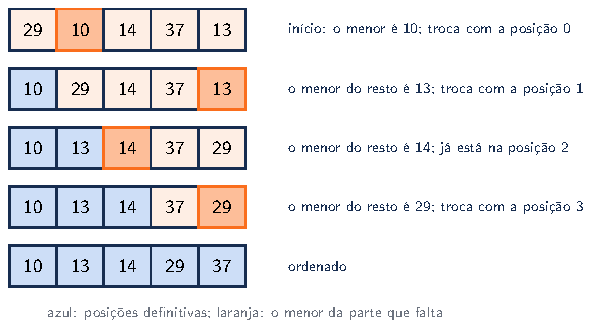
\includegraphics[width=0.85\linewidth,keepaspectratio]{imagens/capitulo-10_selecao.pdf}
\end{center}

\begin{codigo}
\begin{Verbatim}[breaklines=true, breaksymbolleft={}, fontsize=\footnotesize]
void selecao(int v[], int n) {
    for (int i = 0; i < n - 1; i++) {
        int iMenor = i;                       // procura o menor
        for (int j = i + 1; j < n; j++) {     // no resto
            if (v[j] < v[iMenor]) iMenor = j;
        }
        swap(v[i], v[iMenor]);                // e o põe em i
    }
}
\end{Verbatim}
\end{codigo}

O padrão do menor elemento é o do Capítulo 7, aplicado à parte do vetor que ainda não está ordenada. Em Portugol, com o vetor de 1 a \texttt{n} e a troca feita por uma variável auxiliar:

\begin{codigo}
\begin{Verbatim}[breaklines=true, breaksymbolleft={}, fontsize=\footnotesize]
algoritmo "OrdenacaoPorSelecao"
var
   v: vetor[1..5] de inteiro
   i, j, iMenor, aux: inteiro
inicio
   para i de 1 ate 5 faca
      leia(v[i])
   fimpara
   para i de 1 ate 4 faca
      iMenor <- i
      para j de i + 1 ate 5 faca
         se v[j] < v[iMenor] entao
            iMenor <- j
         fimse
      fimpara
      aux <- v[i]
      v[i] <- v[iMenor]
      v[iMenor] <- aux
   fimpara
   para i de 1 ate 5 faca
      escreva(v[i], " ")
   fimpara
fimalgoritmo
\end{Verbatim}
\end{codigo}

A primeira passada faz $n - 1$ comparações, a segunda $n - 2$, e assim por diante, num total de $n(n-1)/2$: para mil elementos, quase meio milhão. Esse número é sempre o mesmo, esteja o vetor bagunçado ou já ordenado. Em compensação, a seleção faz no máximo $n - 1$ trocas, o que é uma vantagem quando trocar elementos é caro.

\subsection{10.5 Ordenação por bolha}

A \textbf{ordenação por bolha} (\textit{bubble sort}) compara cada par de elementos vizinhos e os troca quando estão fora de ordem. Ao fim da primeira passada, o maior elemento ``borbulhou'' até a última posição; na segunda, o segundo maior chega à penúltima, e assim por diante. Se uma passada inteira termina sem nenhuma troca, o vetor já está ordenado e o algoritmo pode parar.

\begin{codigo}
\begin{Verbatim}[breaklines=true, breaksymbolleft={}, fontsize=\footnotesize]
void bolha(int v[], int n) {
    for (int fim = n - 1; fim > 0; fim--) {
        bool trocou = false;
        for (int j = 0; j < fim; j++) {     // até o fim atual
            if (v[j] > v[j + 1]) {          // fora de ordem
                swap(v[j], v[j + 1]);
                trocou = true;
            }
        }
        if (!trocou) break;                 // já está ordenado
    }
}
\end{Verbatim}
\end{codigo}

Graças ao \texttt{trocou}, um vetor que já está ordenado é verificado com uma única passada, de $n - 1$ comparações. Em um vetor bagunçado, porém, a bolha faz tantas comparações quanto a seleção e muito mais trocas, e costuma ser o mais lento dos três algoritmos deste capítulo. Ela é estudada por ser simples, não por ser boa.

\subsection{10.6 Ordenação por inserção}

A \textbf{ordenação por inserção} imita outra forma de ordenar cartas: recebe-se uma carta de cada vez e insere-se cada uma no lugar certo entre as que já estão na mão, que permanecem ordenadas. No vetor, a parte da esquerda é a ``mão'' ordenada. A cada passo, o próximo elemento é guardado em \texttt{atual}, os maiores que ele são deslocados uma posição para a direita, abrindo espaço, e \texttt{atual} entra no buraco aberto.

\begin{center}
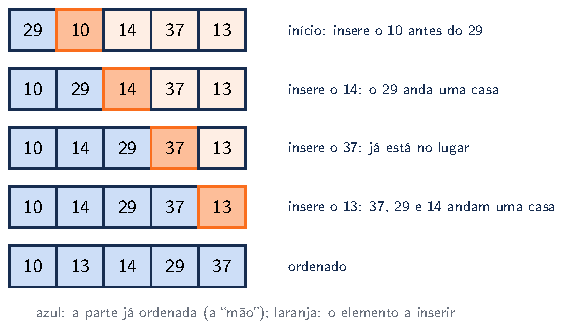
\includegraphics[width=0.85\linewidth,keepaspectratio]{imagens/capitulo-10_insercao.pdf}
\end{center}

\begin{codigo}
\begin{Verbatim}[breaklines=true, breaksymbolleft={}, fontsize=\footnotesize]
void insercao(int v[], int n) {
    for (int i = 1; i < n; i++) {
        int atual = v[i];                   // a carta da vez
        int j = i - 1;
        while (j >= 0 && v[j] > atual) {    // os maiores andam
            v[j + 1] = v[j];                // uma casa à direita
            j--;
        }
        v[j + 1] = atual;                   // entra no buraco
    }
}
\end{Verbatim}
\end{codigo}

A ordem das condições no \texttt{while} importa: \texttt{j >= 0} vem primeiro para que, quando \texttt{j} chegar a $-1$, o \texttt{\&\&} pare antes de acessar \texttt{v[-1]} (avaliação em curto-circuito, Seção 3.6).

A inserção tem uma qualidade especial: o laço de dentro para assim que encontra um elemento menor que \texttt{atual}. Em um vetor quase ordenado, cada elemento anda pouco, e o algoritmo fica muito rápido, perto de $n$ comparações. Em um vetor bagunçado, faz em média metade das comparações da seleção. Por isso, entre os algoritmos simples, ela costuma ser a melhor escolha, e é usada até dentro de algoritmos sofisticados para ordenar trechos pequenos.

\subsection{10.7 Comparando os algoritmos e usando a biblioteca}

O programa abaixo põe as três ordenações para trabalhar sobre os mesmos dados e conta as comparações de cada uma. Os vetores são sorteados com o gerador de números aleatórios da biblioteca \texttt{<random>}, e cada função recebe um \texttt{vector} \textbf{por valor}, ou seja, uma cópia, para que todas ordenem os mesmos números.

\begin{codigo}
\begin{Verbatim}[breaklines=true, breaksymbolleft={}, fontsize=\footnotesize]
#include <iostream>
#include <vector>
#include <random>
#include <algorithm>     // sort
#include <iomanip>       // setw
#include <string>
using namespace std;

long long selecao(vector<int> v) {
    long long comp = 0;
    int n = v.size();
    for (int i = 0; i < n - 1; i++) {
        int iMenor = i;
        for (int j = i + 1; j < n; j++) {
            comp++;
            if (v[j] < v[iMenor]) iMenor = j;
        }
        swap(v[i], v[iMenor]);
    }
    return comp;
}

long long bolha(vector<int> v) {
    long long comp = 0;
    int n = v.size();
    for (int fim = n - 1; fim > 0; fim--) {
        bool trocou = false;
        for (int j = 0; j < fim; j++) {
            comp++;
            if (v[j] > v[j + 1]) {
                swap(v[j], v[j + 1]);
                trocou = true;
            }
        }
        if (!trocou) break;
    }
    return comp;
}

long long insercao(vector<int> v) {
    long long comp = 0;
    int n = v.size();
    for (int i = 1; i < n; i++) {
        int atual = v[i];
        int j = i - 1;
        while (j >= 0) {
            comp++;
            if (v[j] <= atual) break;
            v[j + 1] = v[j];
            j--;
        }
        v[j + 1] = atual;
    }
    return comp;
}

int main() {
    mt19937 gerador(2026);                    // semente fixa
    uniform_int_distribution<int> sorteio(1, 1000000);
    cout << "    n  dados        seleção    bolha  inserção"
         << endl;
    for (int n = 1000; n <= 4000; n *= 2) {
        vector<int> v(n);
        for (int &x : v) x = sorteio(gerador);
        for (int vez = 1; vez <= 2; vez++) {
            string dados = vez == 1 ? "aleatório" : "ordenado ";
            cout << setw(5) << n << "  " << dados << "  "
                 << setw(9) << selecao(v) << setw(9) << bolha(v)
                 << setw(10) << insercao(v) << endl;
            sort(v.begin(), v.end());    // 2a vez: v ordenado
        }
    }
    return 0;
}
\end{Verbatim}
\end{codigo}

Compilado com o g++, o programa mostra a saída abaixo. Como a semente do gerador é fixa (2026), os números sorteados são sempre os mesmos; outro compilador pode sortear outros, e as contagens da bolha e da inserção mudam um pouco, mas o padrão é o mesmo.

\begin{codigo}
\begin{Verbatim}[breaklines=true, breaksymbolleft={}, fontsize=\footnotesize]
// saída
    n  dados        seleção    bolha  inserção
 1000  aleatório     499500   496872    253165
 1000  ordenado      499500      999       999
 2000  aleatório    1999000  1996515   1030270
 2000  ordenado     1999000     1999      1999
 4000  aleatório    7998000  7990860   3918434
 4000  ordenado     7998000     3999      3999
\end{Verbatim}
\end{codigo}

Repare em três coisas. Quando $n$ dobra, as comparações nos vetores aleatórios quadruplicam: é o crescimento $n^2$ da Seção 10.3. A inserção faz cerca de metade das comparações da seleção. E, no vetor já ordenado, a bolha e a inserção fazem só $n - 1$ comparações, enquanto a seleção continua fazendo todas.

\subsubsection{O sort da biblioteca}

Na prática, ninguém escreve a própria ordenação para usar em um programa: a biblioteca \texttt{<algorithm>} oferece a função \texttt{sort}, que usa um algoritmo $O(n \log n)$, muito mais rápido que os deste capítulo para vetores grandes, e a \texttt{binary\_search}, que faz a busca binária:

\begin{codigo}
\begin{Verbatim}[breaklines=true, breaksymbolleft={}, fontsize=\footnotesize]
#include <iostream>
#include <vector>
#include <algorithm>
using namespace std;

int main() {
    vector<int> v = {42, 7, 19, 73, 4, 56, 23};
    sort(v.begin(), v.end());                     // crescente
    for (int x : v) cout << x << " ";
    cout << endl;                         // 4 7 19 23 42 56 73
    cout << binary_search(v.begin(), v.end(), 56) << endl;   // 1
    int w[] = {5, 2, 9, 1};
    sort(w, w + 4);                               // vetor comum
    cout << w[0] << " " << w[3] << endl;          // 1 9
    return 0;
}
\end{Verbatim}
\end{codigo}

Os algoritmos que fazem $O(n \log n)$ comparações, como a ordenação por intercalação (\textit{merge sort}) e o \textit{quicksort}, usam a ideia de dividir o vetor em partes, ordenar cada parte recursivamente e combinar os resultados. Eles ficam para um estudo mais avançado de estruturas de dados. Estudar os algoritmos simples continua valendo a pena: eles ensinam a raciocinar sobre laços, trocas e custo, e são a base para entender os mais sofisticados.

\subsection{10.8 Um programa completo: classificação da turma}

Em um programa real, os dados ordenados raramente são só números: cada nota pertence a um aluno. Quando nomes e notas estão em dois vetores \textbf{paralelos}, em que \texttt{nomes[i]} e \texttt{notas[i]} são do mesmo aluno, a ordenação precisa trocar os dois vetores juntos, senão os nomes se separam das notas. O programa abaixo monta a classificação da turma, da maior nota para a menor, e depois procura a posição de um aluno.

\begin{codigo}
\begin{Verbatim}[breaklines=true, breaksymbolleft={}, fontsize=\footnotesize]
#include <iostream>
#include <string>
using namespace std;

const int N = 6;

// seleção pela maior nota, levando o nome junto
void ordenarPorNota(string nomes[], double notas[], int n) {
    for (int i = 0; i < n - 1; i++) {
        int iMaior = i;
        for (int j = i + 1; j < n; j++) {
            if (notas[j] > notas[iMaior]) iMaior = j;
        }
        swap(notas[i], notas[iMaior]);
        swap(nomes[i], nomes[iMaior]);    // o nome vai junto
    }
}

int buscarNome(const string nomes[], int n, const string &nome) {
    for (int i = 0; i < n; i++) {
        if (nomes[i] == nome) return i;
    }
    return -1;
}

int main() {
    string nomes[N] = {"Ana", "Bruno", "Carla",
                       "Diego", "Elisa", "Fabio"};
    double notas[N] = {7.5, 9.0, 6.0, 9.5, 8.0, 5.5};
    ordenarPorNota(nomes, notas, N);
    for (int i = 0; i < N; i++) {
        cout << i + 1 << "o lugar: " << nomes[i] << " ("
             << notas[i] << ")" << endl;
    }
    string nome;
    cout << "Posição de quem? ";
    cin >> nome;
    int pos = buscarNome(nomes, N, nome);
    if (pos >= 0) {
        cout << nome << " ficou em " << pos + 1 << "o lugar"
             << endl;
    } else {
        cout << nome << " não está na turma" << endl;
    }
    return 0;
}
// 1o lugar: Diego (9.5)    4o lugar: Ana (7.5)
// 2o lugar: Bruno (9)      5o lugar: Carla (6)
// 3o lugar: Elisa (8)      6o lugar: Fabio (5.5)
// Posição de quem? Elisa  ->  Elisa ficou em 3o lugar
\end{Verbatim}
\end{codigo}

A busca pelo nome é sequencial porque, depois de ordenado por nota, o vetor de nomes não está em ordem alfabética, e a busca binária exigiria isso. Os vetores paralelos funcionam, mas é fácil esquecer de trocar um deles. No Capítulo 11, os dados de cada aluno vão ser reunidos em um único registro, e a ordenação passa a mover o registro inteiro de uma vez.

\subsection{Erros Comuns}

\begin{itemize}
  \item \textbf{Usar a busca binária em um vetor desordenado.} Ela não dá erro: simplesmente responde errado.
  \item \textbf{Errar a atualização dos limites na busca binária.} \texttt{ini = meio} em vez de \texttt{meio + 1} pode deixar o laço preso para sempre.
  \item \textbf{Confundir a posição com o valor.} A busca devolve \textbf{onde} o valor está, e $-1$ (ou 0, no Portugol com índices a partir de 1) quando não acha. Teste esse caso antes de usar a posição.
  \item \textbf{Errar os limites dos laços de ordenação.} Na bolha, \texttt{v[j + 1]} exige \texttt{j < fim}; com \texttt{j <= fim}, o último acesso sai do vetor.
  \item \textbf{Inverter a ordem das condições na inserção.} \texttt{v[j] > atual \&\& j >= 0} acessa \texttt{v[-1]} antes de testar o índice.
  \item \textbf{Ordenar um vetor paralelo e esquecer o outro.} Os nomes deixam de corresponder às notas.
  \item \textbf{Escrever a própria ordenação sem necessidade.} Em programas reais, use \texttt{sort}; os algoritmos simples servem para aprender e para vetores pequenos.
\end{itemize}
